En este capítulo hablaremos del Centro Mexicano para la Producción más Limpia, que es la entidad para la cual se desarrolla el sistema, objeto del trabajo terminal. El CMPL es un órgano del Instituto Politécnico Nacional, el cual tiene que observar normatividad de entes por parte del Gobierno Federal, de la Secretaría de Educación Pública y de órganos internacionales como se explicará a continuación. Describiremos dicha normatividad, las actividades, la organización del CMPL y los sistemas de información con los que cuenta. Dicha descripción está enfocada en el control de la correspondencia ya que es el área que desea atacar este trabajo terminal.

\section{El Centro Mexicano para la Producción más Limpia del Instituto Politécnico Nacional}

	El Centro Mexicano para la Producción más Límpia (CMPL) es una instancia del Instituto Politécnico Nacional (IPN), que se dedica a la investigación y elaboración de procesos de producción más limpia. El CMPL, como dice en su página web:

	\begin{quotation}Es integrante de la red mundial de centros de producción más límpia y de la red latinoamericana de producción más limpia, promovidas por la Organización de las Naciones Unidas para el Desarrollo Industrial (ONUDI) y el Programa de las Naciones Unidas para el Medio Ambiente (PNUMA). Cuenta con 13 años de experiencia realizando trabajo técnico para la industria nacional atendiendo sectores como alimentos, petroquímicos, cementeros, galvanoplastia y embotelladoras, por mencionar algunos. Los servicios que ofrece el CMPL son: diagnóstico en producción más limpia y eficiencia energética, diplomados a distancia, presenciales y Maestría en Producción Más Limpia, realización de proyectos de mecanismo de desarrollo limpio, planes de manejo de residuos y análisis de químicos \cite{PoliticaCMPL}.
	\end{quotation}
	
	Para lograr lo anterior, el CMPL cuenta con los siguientes objetivos:
	
	\begin{itemize}
		\item Llevar a cabo un proceso de mejora continua en todos los ámbitos a través del establecimiento y revisión de objetivos y metas \cite{PoliticaCMPL}.
		\item Tener en cuenta los requisitos establecidos por nuestros clientes \cite{PoliticaCMPL}.
		\item Asumir el compromiso de cumplir los requisitos aplicables, tanto legales y reglamentarios como otros que la organización suscriba \cite{PoliticaCMPL}.
		\item Implicar, motivar y comprometer a todo el personal para que se involucre en la organización, así como su formación, motivación y comunicación \cite{PoliticaCMPL}.
		\item Desarrollar actividades formativas para que todos los integrantes del CMPL conozcan, participen y apliquen el Programa de Protección Civil del IPN \cite{PoliticaCMPL}.
		\item Establecer como uno de nuestros objetivos principales la prevención de la contaminación \cite{PoliticaCMPL}.
		\item Utilizar de modo racional, oportuno, pertinente y adecuado los recursos materiales, fomentar el ahorro energético y la reducción de la producción de residuos\cite{PoliticaCMPL}. 
	\end{itemize}

	Como apoyo para la realización de dichos objetivos, el CMPL tiene objetivos de calidad y del medio ambiente bien definidos. Dichos objetivos están definidos con base a las normas ISO 9001-2008 e ISO 140001, las cuales se abordan más adelante.\\

\textbf{Objetivos de calidad}

\begin{itemize}
	\item Supervisar el cumplimiento del plan operativo anual \cite{PoliticaCMPL}.
	\item Impulsar la maestría en Ingeniería de producción más limpia \cite{PoliticaCMPL}.
	\item Supervisar el cumplimiento con los lineamientos administrativos definidos por el Instituto \cite{PoliticaCMPL}.
	\item Impulsar las actividades de investigación, desarrollo e innovación (I+D+i) de proyectos nacionales o internacionales de producción más limpia y los relacionados con el desarrollo industrial sustentable \cite{PoliticaCMPL}.
 \item Promover la vinculación con el Gobierno, la iniciativa privada a nivel nacional y la vinculación internacional \cite{PoliticaCMPL}.
	\item Fortalecer el Programa Institucional para la Sustentabilidad del IPN \cite{PoliticaCMPL}.
\end{itemize}

\textbf{Objetivos ambientales}

\begin{itemize}
	\item Reducir el consumo de agua un 2.5\% \cite{PoliticaCMPL}.
	\item Reducir un 3\% para el 2014, respecto al consumo de energía eléctrica del 2012 \cite{PoliticaCMPL}.
	\item Reducir el consumo de papel un 5\% \cite{PoliticaCMPL}.
	\item Mantener el Programa para la Gestión Integral de Residuos \cite{PoliticaCMPL}.
	\item Realizar el mantenimiento del transformador cada dos años \cite{PoliticaCMPL}.
\end{itemize}

	Con todo lo anterior, el CMPL requiere estar certificado por las normas ISO 9001:2008 (para la calidad) y la norma ISO 14001 (para el medio ambiente). Para lograr dichas certificaciones, el CMPL cuenta con un Sistema Integral de Gestión para la Calidad y el Medio Ambiente. Dicho sistema se denomina SIG y garantiza que el CMPL cumple con todos los lineamientos requeridos para ser considerado un centro de producción más limpia de calidad. Sin embargo, existen otras normas aplicables que se deben considerar, las cuales serán explicadas a continuación.
	
\section{Normatividad}
	En esta sección hablaremos de la normatividad que contemplamos para este proyecto, ya que es importante saber lo que dicen estas normas y cómo son aplicadas dentro de los procedimientos y servicios del CMPL para la implementación del sistema de información.\\
	
	\subsection{Manual de procedimientos para el manejo de la correspondencia y archivo en las Unidades responsables del Instituto Politécnico Nacional}
	
	El manual de procedimientos para el manejo de la correspondencia y archivo en las Unidades responsables del Instituto Politécnico Nacional, es un documento que sienta las bases para el desarrollo coherente y homogéneo de las actividades inherentes a la administración de la documentación en las unidades responsables del IPN, que resuelve efectivamente las demandas al respecto. Su objetivo es proporcionar a las áreas de correspondencia y archivo de las unidades responsables del IPN un instrumento técnico administrativo que contenga los principales procedimientos para la recepción, seguimiento, organización, conservación,
transferencia, préstamo, selección y control de la documentación manejada por la unidad, así como de la generada por la misma \cite{ManProcyArcIPN}.\\
	
	Este manual contiene los procedimientos permitidos para la revisión, recepción, registro y control de correspondencia de entrada y salida de todas las unidades responsables del IPN, por lo que es necesario conocer dichos procedimientos, de manera que el sistema de este trabajo terminal responda a dichos procedimientos, permitiendo al CMPL continuar con lo establecido en el manejo de correspondencia.\\
	
	Los procedimientos que dicta este manual son:\\
	
	\begin{itemize}
		\item \textbf{Revisión, recepción, registro y control de correspondencia de entrada}: Contribuir a que en las unidades responsables del Instituto se realicen de manera expedita y eficiente la revisión, recepción, registro y control de la correspondencia que ingresa a la misma, para evitar demoras en el desahogo de los trámites de su competencia\cite{ManProcyArcIPN}.
		\item \textbf{Clasificación, catalogación y apertura de expedientes de archivo en trámite}: Clasificar, catalogar e integrar los expedientes correspondientes a la documentación de la unidad responsable para agilizar su localización, seguimiento y archivación\cite{ManProcyArcIPN}.
		\item \textbf{Control de correspondencia en trámite}: Llevar un efectivo seguimiento y control de la documentación de las unidades responsables del Instituto para el correcto y oportuno desahogo de los trámites y asuntos de su competencia\cite{ManProcyArcIPN}.
		\item  \textbf{Análisis de trámite, expurgo y glosa de documentos}: Organizar y preservar en forma ordenada los antecedentes documentales de las gestiones realizadas por la unidad responsable para su efectivo aprovechamiento y consulta\cite{ManProcyArcIPN}.
		\item  \textbf{Préstamo de expedientes activos}: Brindar el apoyo informativo indispensable a los órganos que conforman a la unidad responsable, así como a personas externas a ella que lo soliciten para la correcta y oportuna atención de las actividades cotidianas\cite{ManProcyArcIPN}.
		\item  \textbf{Recepción, caracterización, registro, tasa, franqueo y despacho de correspondencia de salida}: Distribuir la documentación generada por la unidad responsable para garantizar que sea recibida oportuna y completamente por sus destinatarios, en el contexto del proceso continuo de tramitación y comunicación intra y extrainstitucional\cite{ManProcyArcIPN}.
		\item  \textbf{Registro y tramitación de transferencia primaria y recepción de documentación concentrada}: Detectar y transferir sistemáticamente la documentación archivada que deja de tener utilidad inmediata en la atención de los trámites de la unidad responsable para que el manejo sea más eficiente y racional\cite{ManProcyArcIPN}.
		\item  \textbf{Préstamo de expedientes concentrados en el archivo general del instituto}: Prestar y proporcionar los expedientes concentrados en el Archivo General del Instituto, a los usuarios que lo soliciten para contribuir eficazmente al desarrollo de sus actividades\cite{ManProcyArcIPN}.
		\item  \textbf{Cancelación de documentación semiactiva}: Retirar oportunamente los materiales documentales de las unidades responsables, cuya utilidad primaria haya prescrito y que carecen de la importancia que justifique su ulterior conservación para asegurar la preservación de aquellos con valor permanente\cite{ManProcyArcIPN}.
	\end{itemize}
	
	Este manual de procedimientos, como se mencionó anteriormente, es aplicable a todo el IPN. Sin embargo, el CMPL, al ser un centro de investigación y producción más limpia necesita tener procedimientos que sean más comprometidos con el medio ambiente y la calidad. Por esta razón, en conjunto con la Dirección de Planeación del IPN, el CMPL diseñó su propio manual para estos procedimientos, mismo que se describe en seguida.	
	
	\subsection{Manual de Procedimientos del Centro Mexicano para la Producción más Limpia}
	El Manual de Procedimientos del Centro Mexicano para la Producción más Limpia, es un instrumento que se basa en el manual de procedimientos tipo de los Centros de Investigación, para su realización se contó la asesoría de la Dirección de Planeación. El propósito del manual es promover la realización ordenada y eficiente de las actividades del Centro Mexicano para la Producción más Limpia con el fin de ofrecer servicios ágiles, efectivos, con el firme objeto de mantener al día sus esquemas de operación y control\cite{ManProcCMPL}.\\
	
	Para el presente trabajo terminal, nos enfocaremos en los procedimientos para el control y gestión administrativa de documentos del CMPL, mismo que se describe a continuación.\\
	
		\subsubsection{Control y gestión administrativa de documentos}
	
	El propósito de este procedimiento es realizar el control y gestión de los documentos que ingresan y se generan al interior de la unidad responsable, para brindar atención expedita y oportuna a las instancias que lo requieran. Este procedimiento es de aplicación generalizada y obligatoria para todo el personal que tiene asignada alguna actividad en el control y gestión administrativa de documentos en el Centro Mexicano para la Producción más Limpia\cite{ManProcCMPL}.\\
	
		\textbf{Políticas de operación}\\
		
	Se describen a continuación, de manera generalizada, las políticas que se deben cumpli al momento de manejo de archivos y correspondencia dentro del CMPL.
		
		\begin{enumerate}
			\item La correspondencia que ingrese, dirigida al Director del Centro Mexicano para la Producción más Limpia (CMP+L), deberá ser registrada y controlada, a través del control de correspondencia de la intranet\cite{ManProcCMPL}.
			\item La correspondencia gestionada en la unidad responsable, recibirá el tratamiento que se indica en la Ley Federal de Transparencia y Acceso a la Información Pública Gubernamental\cite{ManProcCMPL}.
			\item Los documentos que ingresen al Centro Mexicano para la Producción más Limpia, deberán estar firmados por el remitente y con el sello correspondiente de la entidad que envía; si contiene anexo archivo magnético, se comprobará que contenga la información descrita en el documento; si menciona anexos, se verificará que estén completos\cite{ManProcCMPL}.
			\item El documento original deberá escanearse y subirse al apartado de oficios recibidos dentro de la aplicación de control de correspondencia de la intranet\cite{ManProcCMPL}.
		\end{enumerate}
		
	La figura \ref{fig:FlujoCMPL} muestra el diagrama de flujo que describe el proceso de correspondencia y manejo de archivo que sigue el CMPL según las políticas anteriores.		
		
	\begin{figure}[htbp!]
		\centering
			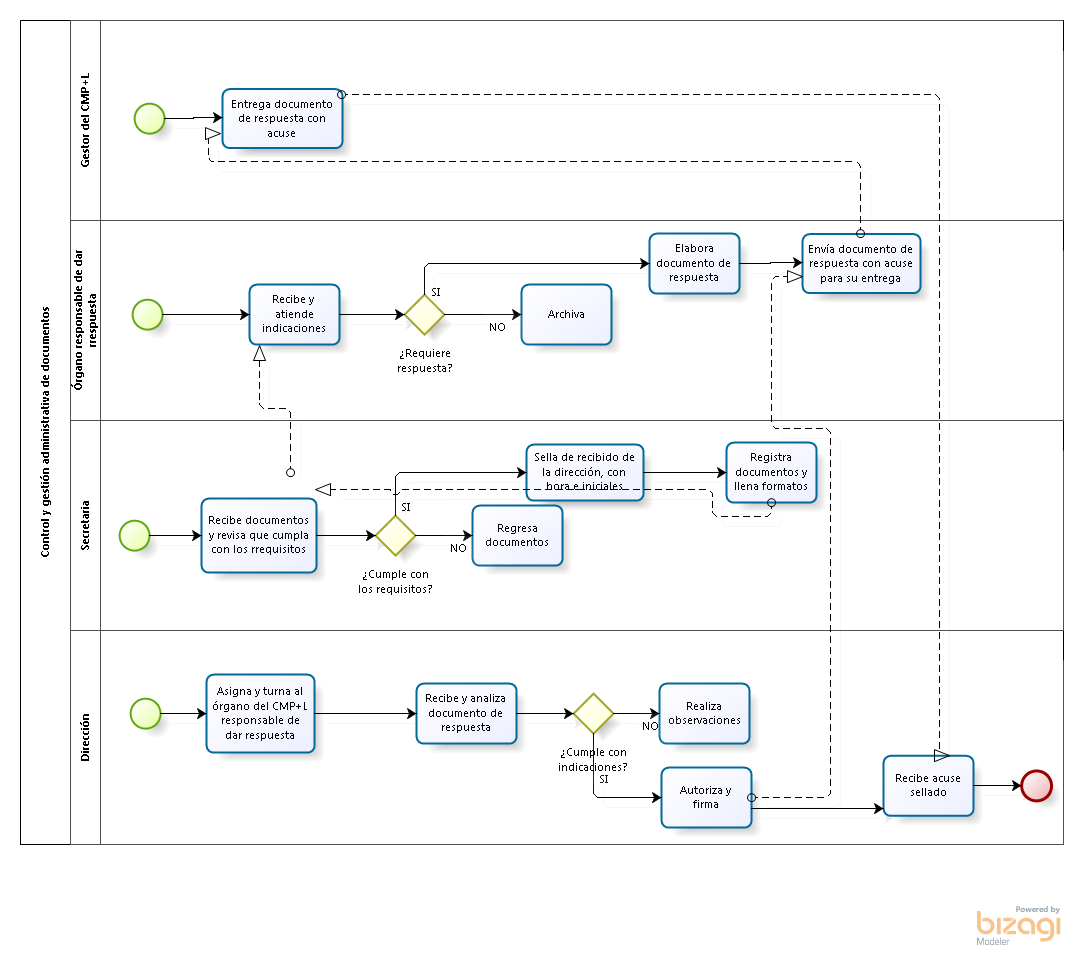
\includegraphics[width=1.2\textwidth]{images/diagramacmpl.png}
		\caption{Proceso de control de correspondencia y manejo de archivos.}
		\label{fig:FlujoCMPL}
	\end{figure}
	
	El diagrama actúa de la siguiente forma:
	
	\begin{enumerate}
		\item Recibe documentos y revisa que cumpla con los requisitos establecidos en las políticas de operación. ¿Cumple con los requisitos?
		\item No, regresa documentos y/o información. Pasa a la actividad 1.
		\item Si, sella de recibido de la Dirección indica sus iniciales de quién recibió el documento y hora de recepción.
		\item Registra documentos en el apartado de control de correspondencia del intranet y registra si contienen anexos y o archivos magnéticos, posteriormente los pasa a revisión de la dirección.
		\item Asigna y turna al órgano del CMP+L que dará atención al documento.
		\item Recibe y atiende indicaciones. ¿Requiere respuesta?
		\item No, archiva y pasa al fin del procedimiento.
		\item Sí, elabora documento de respuesta.
		\item Recibe y analiza documento de respuesta. ¿Cumple con las indicaciones?
		\item  No, realiza observaciones. Pasa a la actividad 6.
		\item Si, Autoriza, firma y lo turna al órgano que atendió.
		\item  Envía documento de respuesta con su respectivo acuse a oficialía de partes para su entrega ante la instancia correspondiente.
		\item Entrega oficio o memorándum firmado y/o documento de respuesta a la instancia correspondiente y se asegura de que el acuse sea debidamente sellado.
		\item Recibe acuse de recibido y archiva.
		\item Termina proceso.
	\end{enumerate}
	
	Aunque este es el actual procedimiento del CMPL para el control de la correspondencia, es importante saber también cuál es el conjunto de normas que rigen los sistemas de información del CMPL y del IPN , ya que se busca sistematizar computacionalmente este procedimiento, para lo cual debemos abordar un poco de lo que es MAAGTIC-SI, el conjunto de normas y estándares aplicables a las entidades públicas del país por parte del Gobierno Federal, para el desarrollo de todo sistema de cómputo.
	
	\subsection{MAAGTIC-SI}%Explicar qué es esa norma, a quién le aplica y por qué es importante para nosotros y qué partes se van a aplicar.
	El MAAGTIC (Manual Administrativo de Aplicación General en Materia de Tecnologías de la Información y Comunicaciones) es un MANUAL que describe 30 procesos de Tecnologías de Información y Comunicaciones, distribuidos en 11 grupos por área de conocimiento o dominio de aplicación. Para cada área de conocimiento se utilizan los principales estándares y mejores prácticas relacionadas\cite{MAAGTICSI}. Fue publicado en el Diario Oficial de la Federación (DOF) el 13 de julio de 2010 y entró en vigor el 20 de agosto del 2010. Su aplicación es obligatoria para toda la Administración Pública Federal (APF). Por dicha razón, este conjunto de procesos (llamado también conjunto de proyectos) es aplicable a los sitemas IPN y por tanto al CMPL, por lo que es fundamental para nosotros conocer en qué área de este conjunto de proyectos cae el sistema del trabajo terminal y así determinar las normas y estándares aplicables que debemos tomar en consideración.\\
	
	La estructura general de MAAGTIC se muestra en la figura \ref{fig:MAAGTIC}. Como se puede observar, MAAGTIC se encuentra dividido en cuatro grandes grupos, los cuales se describen a grandes rasgos a continuación.\\
	
	\begin{figure}[htbp!]
		\centering
			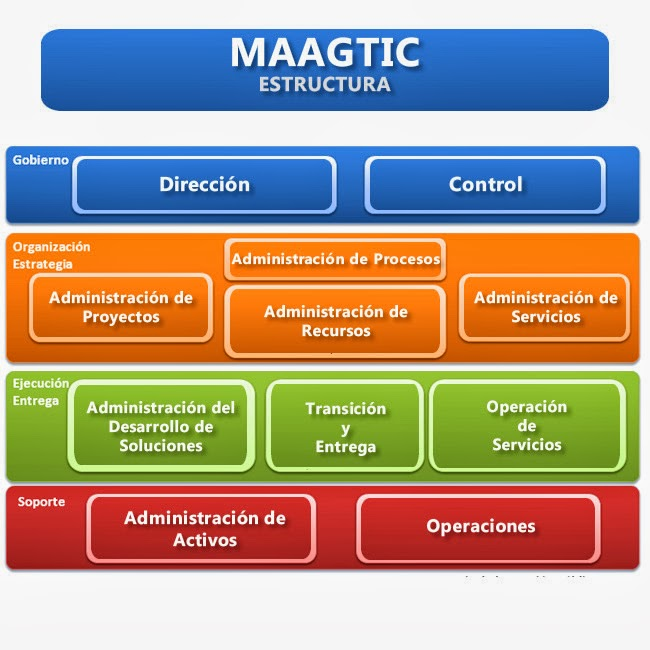
\includegraphics[width=0.6\textwidth]{images/antecedentes/MAAGTICSI.jpg}
		\caption{Estructura de MAAGTIC\cite{MAAGTICSIEstructura}.}
		\label{fig:MAAGTIC}
	\end{figure}
	
	\begin{itemize}
		\item \textbf{Gobierno}: Nivel de gestión que corresponde a los procesos relacionados con la Dirección y el Control en materia de TIC. Este nivel de gestión define, por un lado, los lineamientos de gobernabilidad y estrategia que permiten establecer las líneas de acción en materia de TIC y facilitar la toma de decisiones, y por el otro, establecer los mecanismos de seguimiento y evaluación para disminuir el impacto de eventos adversos\cite{MAAGTICSIGobierno}. El nivel de gestión está conformado por los siguientes grupos:
			\subitem \textbf{Dirección}: El objetivo de la dirección del MAAGTIC consiste en definir los lineamientos de gobernabilidad y estrategia para establecer líneas de acción en materia de TIC\cite{MAAGTICSIGobierno}.
			\subitem \textbf{Control}: Conjunto de procedimientos que permiten establecer mecanismos de seguimiento de la ejecución estratégica, así como directrices para aminorar riesgos de aplicación\cite{MAAGTICSIGobierno}.
		\item \textbf{Organización/Estrategia}: Nivel de gestión que corresponde a los procesos relacionadas con la administración de proyectos, administración de procesos, administración de recursos y la administración de servicios. Este nivel de gestión establece las actividades que permiten la óptima gestión de recursos, su correcta aplicación y verificación, así como de la mejora de los procesos UTIC\cite{MAAGTICSIOrganizacion}. El nivel de gestión está conformado por los siguiente grupos:
			\subitem \textbf{Administración de proyectos}: El objetivo de la administración de proyectos consiste en gestionar las iniciativas de TIC a fin de optimizar la aplicación de los recursos y obtener mayores beneficios en la institución\cite{MAAGTICSIOrganizacion}.
			\subitem \textbf{Administración de procesos}: El objetivo de la administración de procesos consiste en operar un sistema de gestión de los procesos de la UTIC en el que se verifiquen, monitoreen y consideren acciones de mejora\cite{MAAGTICSIOrganizacion}.
			\subitem \textbf{Administración de recursos}: El objetivo de la administración de recursos consiste en coordinar las acciones presupuestales asignadas a las TIC, a fin de maximizar su aplicación en los proyectos y operaciones planeadas\cite{MAAGTICSIOrganizacion}.
			\subitem \textbf{Administración de servicios}: Su objetivo es definir los compromisos y costos de los servicios de las TIC necesarios para el funcionamiento óptimo de la institución, así como la creación de servicios ayuden a cumplir los objetivos estipulados\cite{MAAGTICSIOrganizacion}.
		\item \textbf{Ejecución/Entrega}: Nivel de gestión que corresponde a los procesos relacionadas con la Administración del desarrollo de soluciones, Transición y entrega y Operación de servicios. Este nivel de gestión define requerimientos, desarrolla, valida e integra a la operación las soluciones o servicios tecnológicos de la UTIC\cite{MAAGTICSIEjecucion}. El grupo está conformado por los siguientes procesos:
			\subitem \textbf{Administración y desarrollo de soluciones}: Define los requerimientos necesarios para el desarrollo de soluciones tecnológicas con un marco de referencia sólido para su cumplimiento. Incluye su definición, desarrollo y calidad\cite{MAAGTICSIEjecucion}.
			\subitem \textbf{Transición y entrega}: Su objetivo es planificar y administrar los recursos necesarios para la creación de un servicio nuevo, o bien, modificarlo, enfocándose en minimizar el impacto imprevisto\cite{MAAGTICSIEjecucion}.
			\subitem \textbf{Operación de servicios}: Provee y gestiona los procesos para las operaciones de los servicios de TI, cumpliendo con las estipulaciones y requerimientos del usuario, ya sea en su operación o servicio\cite{MAAGTICSIEjecucion}.
		\item \textbf{Soporte}: Nivel de gestión que corresponde a los procesos relacionadas con la administración de los activos y operaciones. Este nivel de gestión controla y mantiene la operación de la UTIC \cite{MAAGTICSISoporte}. El nivel de gestión está conformado por los siguientes grupos:
			\subitem \textbf{Administración de activos}: Se enfoca a la implementación de arquitecturas tecnológicas efectivas para los denominados dominios tecnológicos, agrupando procesos de administración e integración y desarrollo personal\cite{MAAGTICSISoporte}.
			\subitem \textbf{Operaciones}: El objetivo es establecer los mecanismos para administrar y operar la infraestructura que requiera la entrega de los servicios de TIC que se hayan acordado previamente\cite{MAAGTICSISoporte}.
	\end{itemize}
	
	El proyecto que se presenta en este trabajo terminal está ubicado en la sección de Administración de Proyectos (ADP) de MAAGTIC-SI. ADP se encarga de la planeación, ejecución, monitoreo, control y cierre de los proyectos que el IPN desarrolla y planea implementar en sus procesos, basándose en la norma ISO 9001-2008. Para este trabajo terminal no entraremos de lleno a todo el conjunto de proyectos que se encuetran en la ADP debido al alcance del proyecto, pero sí en los estándares correspondientes a la norma ISO 9001:2008 (calidad) y señalando esta sección como un determinante a considerar en un trabajo a futuro cuando MAAGTIC sea implementado en su totalidad a todos los sistemas del CMPL. En la siguiente sección hablaremos de la norma ISO 9001:2008.	
	
	\subsection{ISO 9001:2008}
	La Norma ISO 9001:2008 elaborada por la Organización Internacional para la Estandarización (ISO), determina los requisitos para un Sistema de Gestión de la Calidad (SGC), que pueden utilizarse para su aplicación interna por las organizaciones, sin importar si el producto o servicio lo brinda una organización pública o empresa privada, cualquiera que sea su tamaño, para su certificación o con fines contractuales.\\
	
	La estructura que tiene esta norma se encuentra diseñada de la siguiente manera.\\
	
	\begin{itemize}
		\item Capítulo 1 al 3: Guías y descripciones generales.
		\item Capítulo 4 Sistema de gestión: contiene los requisitos generales y los requisitos para gestionar la documentación.
		\item Capítulo 5 Responsabilidades de la Dirección: contiene los requisitos que debe cumplir la dirección de la organización, tales como definir la política, asegurar que las responsabilidades y autoridades están definidas, aprobar objetivos, el compromiso de la dirección con la calidad, etc.
		\item Capítulo 6 Gestión de los recursos: la Norma distingue 3 tipos de recursos sobre los cuales se debe actuar: RRHH, infraestructura, y ambiente de trabajo. Aquí se contienen los requisitos exigidos en su gestión.
		\item Capítulo 7 Realización del producto/servicio: aquí están contenidos los requisitos puramente de lo que se produce o brinda como servicio (la norma incluye servicio cuando denomina "producto"), desde la atención al cliente, hasta la entrega del producto o el servicio.
		\item Capítulo 8 Medición, análisis y mejora: aquí se sitúan los requisitos para los procesos que recopilan información, la analizan, y que actúan en consecuencia. El objetivo es mejorar continuamente la capacidad de la organización para suministrar productos y/o servicios que cumplan con los requisitos.
	\end{itemize}
	
	El objetivo declarado en la Norma, es que la organización busque sin descanso la satisfacción del cliente a través del cumplimiento de los requisitos. \cite{ISO9001}\\
	
	Con la ISO 9001, el CMPL garantiza que sus procedimientos generen resultados basados en estándares internacionales, permitiendo así un mejor desarrollo de:\\

	\begin{itemize}
		\item Diagnósticos: El CMPL realiza visitas de reconocimiento a los clientes que deseen hacer sus procesos de producción de una forma más amigable con el medio ambiente, elaborando al final una propuesta técnico-económica que le permita eficientar sus procesos; si el cliente no está de acuerdo con los resultados entonces se cierra el diagnóstico, se presenta una nueva propuesta o se ofrecen otros servicios.
		\item Capacitaciones: El CMPL ofrece varios cursos de capacitación para manejo de residuos y químicos al sector público y privado, con el fin de promover la producción más limpia.
		\item Maestría de Producción más Limpia: El CMPL creó esta Maestría para formar especialistas que se involucren en el análisis de las etapas productivas de cualquier proceso, desde la selección de materias primas, insumos, tecnologías, hasta las emisiones contamintantes del proceso (líquidas, gases, residuos, etc.), así como los impactos ambientales de los productos y servicios. \cite{CMPLWebPage}
	\end{itemize}
	
	Aún cuando el CMPL trabaja sus procedimientos con la ISO 9001:2008, al ser un centro de investigación en Producción más Limpia, se apoya también de la norma ISO 14000 para llevar todos esos procedimientos de una forma más ecológica como la reducción de papel, ahorro de energía eléctrica y apoyo de tecnologías de la información para mitigar el impacto ambiental que todo centro genera. Dicha norma se describe a continuación.
	
	\subsection{ISO 14000}
	La norma ISO 14000 es un estándar internacional de gestión ambiental que se comenzó a publicar en 1996, tras el éxito de la serie de normas ISO 9000 para sistemas de gestión de la calidad. La norma ISO 14000 es una norma internacionalmente aceptada que expresa cómo establecer un Sistema de Gestión Ambiental (SGA) efectivo. La norma ISO 14000 va enfocada a cualquier organización, de cualquier tamaño o sector, que esté buscando reducir los impactos en el ambiente y cumplir con la legislación en materia ambiental.\\
	
	La norma ISO 14000 es un conjunto de documentos de gestión ambiental que, una vez implantados, afectará todos los aspectos de la gestión de una organización en sus responsabilidades ambientales y ayudará a las organizaciones a tratar sistemáticamente asuntos ambientales, con el fin de mejorar el comportamiento ambiental y las oportunidades de beneficio económico. Los estándares son voluntarios, no tienen obligación legal y no establecen un conjunto de metas cuantitativas en cuanto a niveles de emisiones o métodos específicos de medir esas emisiones. Por el contrario, ISO 14000 se centra en la organización proveyendo un conjunto de estándares basados en procedimientos y unas pautas desde las que una empresa puede construir y mantener un sistema de gestión ambiental. \cite{ISO14000}\\
	
	La norma se compone de 8 elementos, los mismos que se relacionan a continuación con su respectivo número de identificación:\\
	
	\begin{itemize}
		\item Sistemas de Gestión Ambiental (14001 Especificaciones y directivas para su uso – 14004 Directivas generales sobre principios, sistemas y técnica de apoyo).
		\item Auditorías Ambientales (14010 Principios generales- 14011 Procedimientos de auditorías, Auditorías de Sistemas de Gestión Ambiental- 14012 Criterios para certificación de auditores).
		\item Evaluación del desempeño ambiental (14031 Lineamientos- 14032 Ejemplos de Evaluación de Desempeño Ambiental).
		\item Análisis del ciclo de vida (14040 Principios y marco general- 14041 Definición del objetivo y ámbito y análisis del inventario- 1404).
	\end{itemize}

	Para apegarse esta norma, el CMPL cuenta con procedimientos para mitigar los impactos ambientales en la elaboración de todas sus actividades. Dichos procedimientos están divididos por subdirecciones y jefaturas, en un documento llamado "Manual de Procedimientos", en donde se describe, según ISO 14000, la forma en la que estas áreas del CMPL deben operar. Incluyen procedimientos para: la reducción de papel en la elaboración de documentos escritos; cuándo se deben sacar copias de ellos o cuándo es más viable compartirlo por correo electrónico y otros medios informáticos; el tiempo de inactividad de los equipos de cómputo antes de entrar en modo de ahorro de energía; configuraciones recomendadas para ahorro de energía en impresoras, scanners, fotocopiadoras, cámaras de video, servidores, pantallas, televisiones, aire acondicionado, microondas, refrigerador, expendedor de agua, no-breaks y sites; en otras palabras, todo lo relacionado a las diversas actividades del CMPL.\\
	
	Para la elaboración del trabajo terminal se tomaron en cuenta dichos procedimientos durante el análisis. En la siguiente sección se describirán las actividades del CMPL, explicando la forma en la que se aplican estas normas.
	
\section{Actividades del CMPL}
	Como toda instancia del IPN, el CMPL debe tener una organización que le permita coordinar todas las actividades de manera que cumplan con lo establecido en el SIG. Su organización está establecida como se muestra en la figura \ref{fig:organigrama}, que es una estructura jerárquica.\\
	
	\begin{figure}[htbp!]
		\centering
			\includegraphics[width=1.2\textwidth]{images/Organigrama.png}
		\caption{Organigrama interno del CMPL. \cite{Organigrama}}
		\label{fig:organigrama}
	\end{figure}
	
	El CMPL cuenta con una dirección, tres subdirecciones y cuatro jefaturas, dos de los cuales están dentro de una subdirección. Cada subdirección y departamento debe entregar indicadores cada mes a la Dirección y una relación donde especifique los objetivos logrados durante el mes; esto con la finalidad de cumplir con la norma ISO 9001:2008 para mejorar la calidad con la que el CMPL trabaja, buscando mejorarla con base en los indicadores de cada subdirección o departamento.\\
	
	\subsection{Objetivos de calidad}
	Para que lo anterior sea posible, cada subdirección y jefatura tiene sus manuales de procedimientos, mismos que deben ser revisados por la Dirección y que deben estar disponibles en todo momento para el personal administrativo y de apoyo del CMPL. La razón de llevar esto a cabo es que de cada subdirección y departamento se conozcan sus diversas actividades y funciones que tienen dentro del CMPL, de forma que se cumplan con sus objetivos de calidad, mismos que se enlistan a continuación.\\
	
	\begin{itemize}
		\item Dirección: Decidir qué se hace y el rumbo que toma el CMPL en función de los lineamientos que cada departamento o jefatura cumple con base en sus indicadores proporcionados cada mes, apoyados siempre de la ISO 9001:2008 e ISO 14000.
		\item Subdirección Técnica: Realizar proyectos de Producción Más Limpia y Eficiencia Energética, que  ayuden a las empresas a prevenir y disminuir la generación de residuos, así como propiciar el uso eficiente de sus recursos. \cite{SIGTecnica}
		\item Subdirección de Vinculación y Apoyo: Los servicios del CMPL, realizar prospección para incrementar la cartera de clientes, así como establecer y mantener el contacto con los clientes. \cite{SIGVinculacion}
		\item Subdirección de Posgrado: Formar recursos humanos en producción más limpia, eficiencia energética y otros temas relacionados con el desarrollo sustentable. \cite{SIGPosgrado}
		\item Jefatura de Servicios Administrativos: Administrar los recursos asignados al CMPL. \cite{SIGAdministrativa}
		\item Departamento de Sistemas y Banco de Datos: Realizar el PEDMP y POA, así como sus seguimientos trimestrales. Coordinar las actividades de los RD's de los diferentes sistemas del CMPL. \cite{SIGSistemas}
	\end{itemize}
	
	En el manual de procedimientos se describen todos los procesos de todas las áreas del CMPL. Para fines del presente trabajo terminal, a continuación describiremos únicamente el proceso de control de correspondencia.
	
	\subsection{Proceso de control de correspondencia}
	El proceso de control de correspondencia se divide en cuatro tipos: oficios entrantes, oficios de respuesta, oficios salientes y memorándums. Los procesos de cada uno de estos subprocesos de control de correspondencia se describen a continuación.\\
	
	El personal involucrado para el proceso de control de correspondencia es llevado a cabo por la  Dirección, Oficialía de Partes, Subdirecciones y Jefaturas. Los siguientes diagramas de procesos describen cada uno de ellos.\\
	
	\subsubsection{Oficios entrantes}
	La figura \ref{fig:OficiosEntrantes} muestra cómo es el proceso de recepción de oficios externos al CMPL y cómo es que éstos son atendidos. El proceso es así:
	
	\begin{enumerate}
		\item Oficialía de Partes recibe oficio entrante.
		\item Oficialía de partes verifica que el oficio recibido cumpla con todos los elementos establecidos en el manual de procedimientos del CMPL.
		\item Si cumple con todos los lineamientos firma de recibido y otorga acuse de recibido.
		\item Sino entonces regresa al portador oficio entrante con las observaciones encontradas que impidieron la recepción del documento y sus anexos. Termina proceso.
		\item Oficialía de Partes registra en la bitácora de control de oficios el oficio que acaba de recibir con su número de oficio externo, fecha, datos de la instancia y encargado que lo emitió y su asunto.
		\item Oficialía de Partes turna el original al Director.
		\item El Director revisa el oficio entrante y checa si es destinado a él.
		\item Si es para él entonces lo atiende.
		\item Sino entonces verifica si el oficio es público, privado o confidencial.
		\item Si el oficio es confidencial entonces el Director turna directamente al destinatario, que puede ser un jefe, un subdirector o un empleado.
		\item El destinatario recibe el oficio y verifica que sea para él.
		\item Si es para él entonces atiende el oficio. Termina proceso.
		\item Si no es para él entonces turna al Director con una nota diciendo que el oficio fue turnado por equivocación a la persona incorrecta. Regresa al paso 7.
		\item Si el oficio no es confidencial entonces el Director turna al Subdirector o Jefe correspondiente.
		\item El Subdirector o Jefe revisa el oficio y verifica si es público o privado.
		\item Si el oficio es público entonces lo atiende. Termina proceso.
		\item Sino entonces verifica si el oficio es privado y lo turna al empleado correspondiente.
		\item El empleado recibe el oficio y lo revisa.
		\item Si el oficio es para él entonces lo atiende. Termina proceso.
		\item Si el oficio no es para él entonces regresa oficio a su jefe directo. Regresa al paso 15.
		\item Termina proceso.
	\end{enumerate}
	
	\begin{figure}[htbp!]
		\centering
			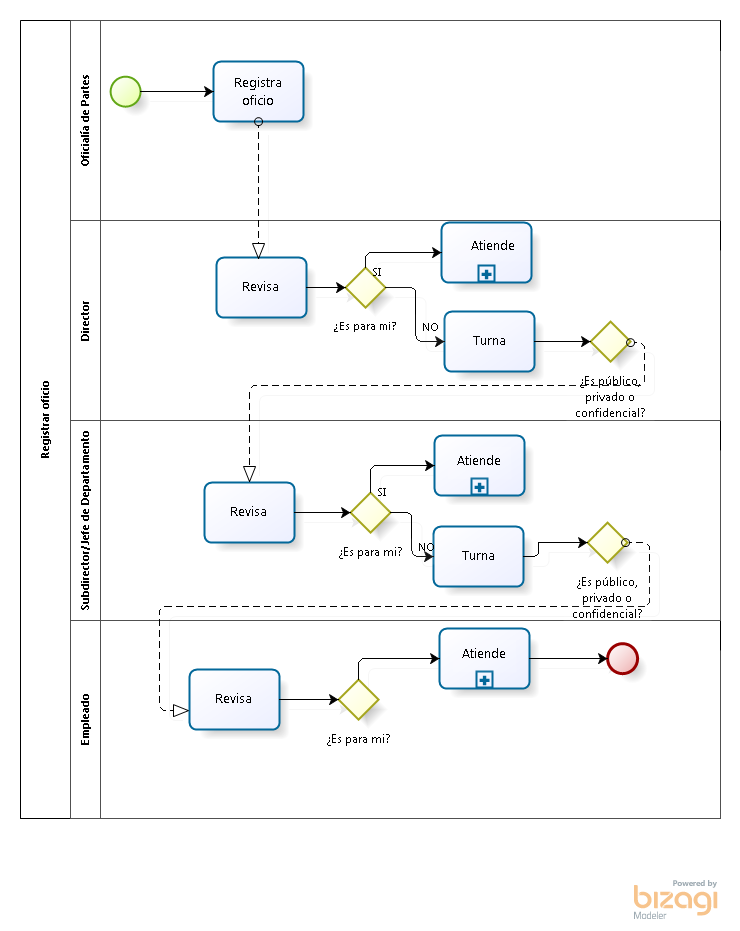
\includegraphics[width=1\textwidth]{images/antecedentes/registraroficio.png}
		\caption{Diagrama de procesos de oficios entrantes.}
		\label{fig:OficiosEntrantes}
	\end{figure}
	
	\subsubsection{Oficios de respuesta}
	La figura \ref{fig:OficiosRespuesta} muestra cómo es el proceso de elaboración, evaluación y envío de oficios externos de respuesta del CMPL. El proceso se describe a continuación.
	
	\begin{enumerate}
		\item El personal (empleado, subdirector, jefe, director) revisa la bitácora de oficios y toma el siguiente número de oficio disponible.
		\item El personal elabora el oficio, anotando el número de oficio al cual se está respondiendo..
		\item El personal turna el oficio a Oficialía de Partes.
		\item Oficialía de Partes recibe el oficio y lo turna al Director.
		\item El Director revisa que cumpla con los lineamientos establecidos en el Manual de Procedimientos del CMPL.
		\item Si cumple con los lineamientos entonces firma el oficio y lo manda a Oficialía de Partes.
		\item Oficialía de Partes envía el oficio y espera acuse de recibido.
		\item Oficialía de Partes recibe acuse de recibido. Termina proceso.
		\item Si no cumple con los lineamientos entonces el Director realiza observaciones y turna oficio de vuelta con observaciones a Oficialía de Partes.
		\item Oficialía de Partes turna de vuelta al personal que realizó dicho oficio.
		\item El personal recibe oficio con correcciones.
		\item El personal realiza correcciones y turna de vuelta a Oficialía de Partes. Regresa al paso 4.
	\end{enumerate}	
	
	\begin{figure}[htbp!]
		\centering
			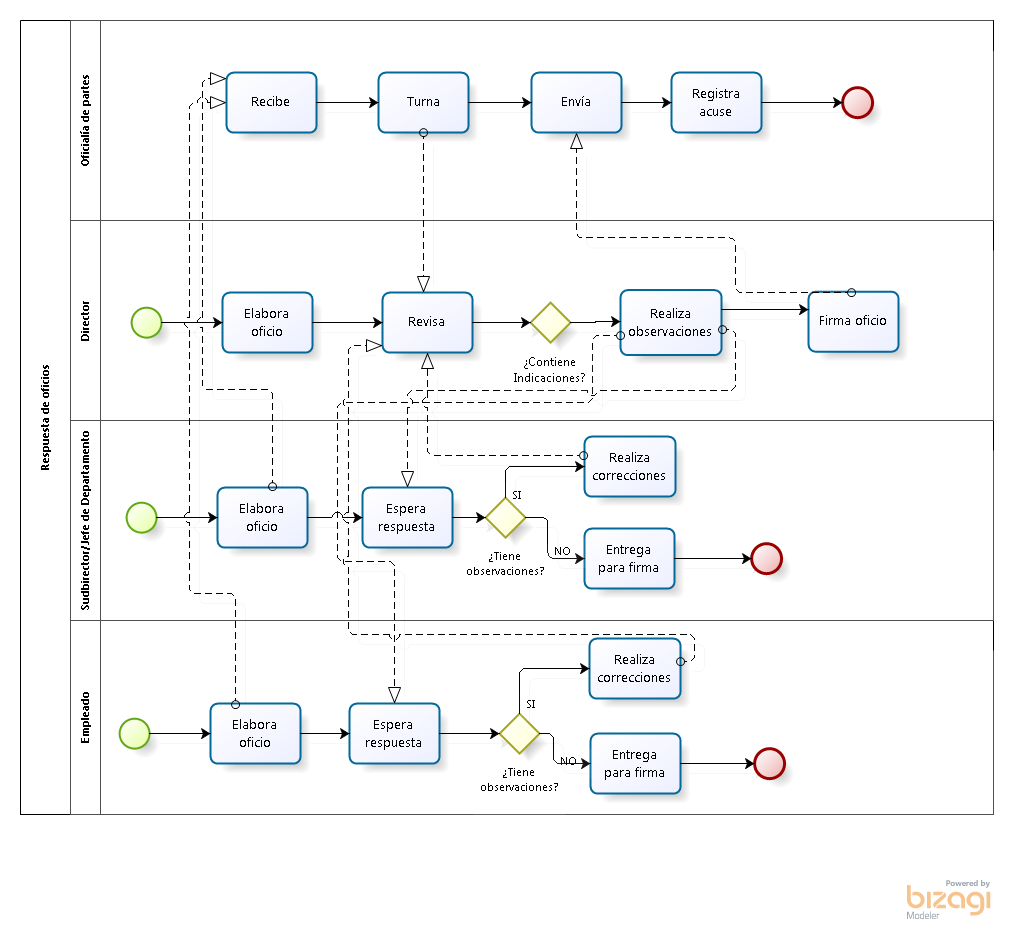
\includegraphics[width=1.2\textwidth]{images/antecedentes/respondeoficio.png}
		\caption{Diagrama de procesos de oficios de respuesta.}
		\label{fig:OficiosRespuesta}
	\end{figure}
	
	\subsubsection{Oficios de salientes}
	La figura \ref{fig:OficiosSalientes} muestra cómo es el proceso de elaboración, evaluación y envío de oficios salientes del CMPL. El proceso es similar al proceso para oficios de respuesta.
	
	\begin{enumerate}
		\item El personal (empleado, subdirector, jefe, director) revisa la bitácora de oficios y toma el siguiente número de oficio disponible.
		\item El personal elabora el oficio.
		\item El personal turna el oficio a Oficialía de Partes.
		\item Oficialía de Partes recibe el oficio y lo turna al Director.
		\item El Director revisa que cumpla con los lineamientos establecidos en el Manual de Procedimientos del CMPL.
		\item Si cumple con los lineamientos entonces firma el oficio y lo manda a Oficialía de Partes.
		\item Oficialía de Partes envía el oficio y espera acuse de recibido.
		\item Oficialía de Partes recibe acuse de recibido. Termina proceso.
		\item Si no cumple con los lineamientos entonces el Director realiza observaciones y turna oficio de vuelta con observaciones a Oficialía de Partes.
		\item Oficialía de Partes turna de vuelta al personal que realizó dicho oficio.
		\item El personal recibe oficio con correcciones.
		\item El personal realiza correcciones y turna de vuelta a Oficialía de Partes. Regresa al paso 4.
	\end{enumerate}
	
	\begin{figure}[htbp!]
		\centering
			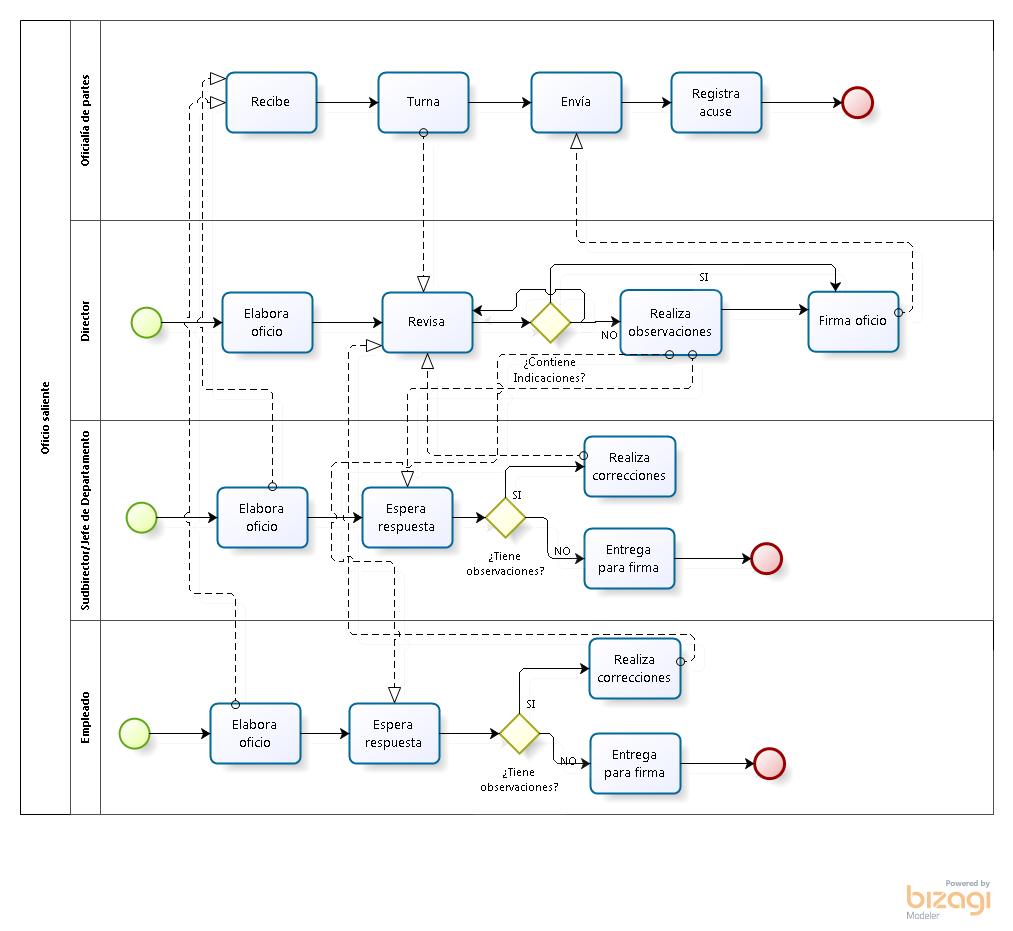
\includegraphics[width=1.2\textwidth]{images/antecedentes/oficiosaliente.png}
		\caption{Diagrama de procesos de oficios salientes.}
		\label{fig:OficiosSalientes}
	\end{figure}

	Aún cuando el CMPL emite y recibe oficios, también tiene procedimientos para el manejo de memorándums interdepartamentales, mismos que se explican a continuación.

\subsection{Memorándums interdepartamentales}
	 Los memorándums interdepartamentales son documentos que comparten información entre los departamentos del CMPL. Existen dos tipos:\\
	
	\begin{itemize}
		\item Memorándums generales: Estos memos van dirigidos a toda la subdirección. Son emitidos por el responsable de cada subdirección o por parte de la dirección. Todo memo general debe ser revisado por el Director antes de ser turnado.
		\item Memorándums personales: Estos memos son de caracter personal y pueden ser enviados de un empleado del CMPL a otro, incluyendo a los Jefes, Subdirectores y al Director. A diferencia de los memos generales, un memo personal no requiere ser revisado por el Director.
	\end{itemize}
	
	Ambos tipos de memorándum pueden contener fechas límites de respuesta y para su emisión es necesario especificar en alguna parte el asunto para poder llevar el control de memorándums. Aunque éstos son diferentes a los oficios, actualmente los manejan como si lo fueran; es decir, se registran en la misma bitácora de oficios y se cuentan como ``Oficios internos''. Sin embargo, sus procesos son más sencillos que los de los oficios. En seguida se describen los procesos del manejo de memorándums dentro del CMPL. 

	\subsubsection{Memorándum general}
	%Hablar de los involucrados en el proceso
	%Describir cada uno de los prcocesos
	%Indicar los requerimientos de las normas
	La figura \ref{fig:MemoGeneral} muestra el proceso para memorándums generales. Dicho proceso se describe a continuación.
	
	\begin{enumerate}
		\item El encargado (Subdirector o Jefe) elabora el memorándum y lo turna a Oficialía de Partes.
		\item Oficialía de Partes lo turna al Director.
		\item El Director lo revisa y evalúa.
		\item Si el memorándum es aprobado por el director entonces el Director turna de vuelta el memorándum a Oficialía de Partes.
		\item Oficialía de Partes turna el memorándum a la subdirección o jefatura correspondiente.
		\item El destinatario (Jefe o Subdirector) recibe el memorándum.
		\item El destinatario verifica que sea para él.
		\item Si es para él entonces firma de recibido y de enterado. Atiende memorándum.
		\item Si no es para él entonces turna de vuelta a Oficialía de Partes. Regresa al paso 5.
		\item Termina proceso.
	\end{enumerate}
	
	%Espacio para meter el diagrama de procesos de memos generales
	
	\subsubsection{Respuesta a memorándum general}
	La figura \ref{fig:MemoReGeneral} muestra el proceso para dar respuesta a memorándums generales. Dicho proceso se describe a continuación.
	
	\begin{enumerate}
		\item El encargado (Subdirector o Jefe) elabora el memorándum de respuesta a memorándum general.
		\item Si tiene identificador el memorándum a responder entonces se anota en el asunto del memorándum de respuesta.
		\item Si no tiene identificador entonces se describe en respuesta a qué memorándum se está contestando.
		\item El encargado elabora el memorándum y lo turna a Oficialía de Partes.
		\item Oficialía de Partes lo turna al Director.
		\item El Director lo revisa y evalúa.
		\item Si el memorándum es aprobado por el director entonces el Director turna de vuelta el memorándum a Oficialía de Partes.
		\item Oficialía de Partes turna el memorándum a la subdirección o jefatura correspondiente que espera la respuesta.
		\item El destinatario (Jefe o Subdirector) recibe el memorándum.
		\item El destinatario verifica que sea para él.
		\item Si es para él entonces firma de recibido y de enterado. Atiende memorándum.
		\item Si no es para él entonces turna de vuelta a Oficialía de Partes. Regresa al paso 5.
		\item Termina proceso.
	\end{enumerate}
	
	\subsubsection{Memoránum personal}
	La figura \ref{fig:MemoPersonal} muestra el proceso para memorándums generales. Dicho proceso se describe a continuación.
	
	\begin{enumerate}
		\item El empleado del CMPL (empleado, Subdirector o Jefe) elabora el memorándum y lo turna a Oficialía de Partes.
		\item Oficialía de Partes lo turna a los debidos destinatarios.
		\item El destinatario (empleado, Subdirector o Jefe) recibe el memorándum.
		\item El destinatario verifica que sea memorándum para él.
		\item Si es para él, el destinarario firman de recibido y de enterado. Atiende memorándum.
		\item El destinatario atiende el asunto del memorándum.
		\item Si no es para él, el destinatario turna de vuelta a Oficialía de Partes. Regresa la paso 2.
		\item Termina proceso.
	\end{enumerate}
	
	\subsubsection{Respuesta a memorándum personal}
	La figura \ref{fig:MemoRePersonal} muestra el proceso para dar respuesta a memorándums personales. Dicho proceso se describe a continuación.
	
	\begin{enumerate}
		\item El empleado del CMPL (empleado, Subdirector o Jefe) elabora el memorándum de respuesta al memorándum personal.
		\item Si tiene identificador el memorándum a responder entonces se anota en el asunto del memorándum de respuesta.
		\item Si no tiene identificador entonces se describe en respuesta a qué memorándum se está contestando.
		\item El empleado elabora el memorándum y lo turna a Oficialía de Partes.
		\item Oficialía de Partes lo turna al destinatario correspondiente.
		\item El destinatario (empleado, Jefe o Subdirector) recibe el memorándum.
		\item El destinatario verifica que sea para él.
		\item Si es para él entonces firma de recibido y de enterado. Atiende memorándum.
		\item Si no es para él entonces turna de vuelta a Oficialía de Partes. Regresa al paso 5.
		\item Termina proceso.
	\end{enumerate}
	
	Toda la información brindada por cada área demanda una cantidad considerable de materia de papelería; el control de oficios y memorándums no queda excento de esta situcación, pues llevar todo ese proceso de forma manual hace que no se tenga un compromiso responsable con el medio ambiente, a la par de que los procesos se vuelven más lentos, afectando la calidad de tranajo del CMPL, incumpliendo con los objetivos de la norma ISO 9001:2008.  En este proceso también entra en juego la norma ISO 14000. Dicha norma exige al CMPL contar con un sistema computacional que automatice en gran parte los procesos del CMPL, buscando reducir la cantidad de papel utilizada, especialmente en documentos que son únicamente de carácter informativo, como lo son generalmente los memorándums. Se describe a continuación el sistema que el CMPL ha implementado como una medida para mitigar el impacto en la calidad del trabajo del CMPL y su compromiso con el medio ambiente.\\
	
	\section{Sistema de información del CMPL}
	El Departamento de Sistemas y Banco de Datos desarrolló un sistema que da soporte en la operación del SIG. Con este sistema se cumplía la reducción del papel y el uso de tecnologías de la información para tener un impacto ambiental más limpio en los procesos del CMPL  y así cubrir parte de los requisitos para obtener la certificación de la ISO 14000. El sistema llevaba como nombre ``Intranet CMPL'', al ser una aplicación web que estaba alojada de forma local en la red del CMPL. Sus funciones eran:\\
	
	\begin{itemize}
		\item Alojar los manuales de procedimientos de cada subdirección y departamento del CMPL, incluyendo sus objetivos específicos y formatos propios de cada subdirección y departamento.
		\item Tener un registro del directorio del CMPL de forma global y por subdirección o departamento. 
		\item Alojamiento de indicadores mensuales por subdirección y departamento para su consulta en las auditorías internas y externas.
		\item Organigrama interno del CMPL.
		\item Formatos de adquisición y requisición de material diverso para el CMPL.
		\item Galería fotográfica con evidencia de los diferentes congresos, expediciones, proyectos y eventos en los que el CMPL ha sido partícipe.
		\item Directorio interno del CMPL.
		\item Sección de avisos de carácter público a todo el personal del CMPL. 
		\item Apartado de software institucional de producción y oficina.
		\item Formatos electrónicos diversos de documentos oficiales, memorándums, circulares y tripticos.
		\item Sección de artículos y reportajes de producción más limpia en el mundo.
		\item Programa de cursos, capacitaciones y servicios que presta el CMPL.
		\item Catálogo de precios de servicios.
		\item Galería de logos oficiales de dependencias con las que el CMPL trabaja.
		\item Control de correspondencia (oficios y memorándums).
	\end{itemize}
	
	Este sistema estaba alojado en un servidor del CMPL, cuyas características eran:
	
	\begin{itemize}
		\item Disco duro de 500 GB.
		\item Memoria RAM de 4 GB.
		\item Sistema Operativo Windows Server 2003.
		\item Servidor web IIS 4.0.
		\item ASP.NET.
		\item Microsoft Office Access 2000.
	\end{itemize}
	
	El por qué este sistema no representa un papel fundamental en el trabajo diario del CMPL se describe a continuación.
		
	\section{Situación actual}
	Este sistema operó hasta abril de 2014, año en el que durante el cambio de administración se perdió la información del sistema y código fuente, a  tal grado que el sistema no pudo volver a operar. A partir de ahí el nuevo personal del CMPL realiza todas sus actividades de forma manual, incumplimiento con la norma ISO 14001. Esto causó que no se recibiera dicha certificación en 2014 y fue la razón por la cual se pensó en volver a desarrollar un nuevo sistema que de soporte al SIG y así poder recuperar la certificación ISO 14000, que es de vital importancia para el CMPL.\\
	
	Esta pérdida de información y recursos obligó al nuevo personal a realizar todas sus actividades de forma manual, generando una serie de complicaciones que dieron paso a los problemas que se describen en el siguiente capítulo.
